\documentclass[12pt] {article}

\usepackage{graphicx}
\usepackage{subfig}


\newcommand{\function}[1]{\texttt{#1}}

\begin{document}

\title{Characterization and Reverse-engineering Assignment - EEC 277}
\author{Ahmed H. Mahmoud}
\date{7 February 2017} 

\maketitle
%========intro====================
\section{Introduction}
This report is divided into two parts; performance analysis of the graphics card and reverse engineering to charactrize undocumneted features of the GPU. In the first part, we are going to characterize the performance of the two GPU using {\fontfamily{qcr}\selectfont wesBench} benchmark. The target here is to find the crossover point between the geometry/vertex stage and fragment/rasterization stage for different scenarios. Broadly speaking, the graphics pipeline overall performance is a function of the slowest of these two stages. It is well known that the geometry stage favors large primitive triangles since the speed of this stage if dependent on the operations-per-triangle. In contrast, rasterization stage favors small primitive triangles since a large triangle would require more fill operations \cite{Bethel_2010}. All the experiments presented in the report are done on NVIDIA GeForce GT 610 GPU on a Windows 7 machine with four-core Intel(R) Xeon(R) CPU of 3.7GHz and 32.0GB RAM.

\section{Geometry Rate Vs. Fill Rate:}
The objective of first experiment is to find the crossover point for the unlit untexture triangles between the fill rate and geometry rate. This is done by testing both rates for different triangle sizes. The results are shown in Figure \ref{fig:fill_geo1}(a) on a log-log scale, where the fill rate (MFrags/Sec) increases as expected for small triangles and geometry rate (MVerts/Sec) decreases. The crossover point is between triangle area between 2 and 4 pixels. We notice that for triangle of size between 2 to 16 pixels the geometry rate is almost constant.  Even though the geometry rate is the highest but this could be due to more efficient use of caching. Since the triangles are of small size, and due to spatial locality, more triangle can be fetched and put into the cache. On the other side, the rapid change on the fill rate starts to slow down at triangle size greater than 16 pixels. This could be due to the fact the geometry stage is not sending enough work for the rasterization stage. So even the overall fill rate increases as the triangle size increases, but the slope of the line is not the same overall.

\begin{figure}[!tbh]
 \centering  
 \subfloat[Default]
    {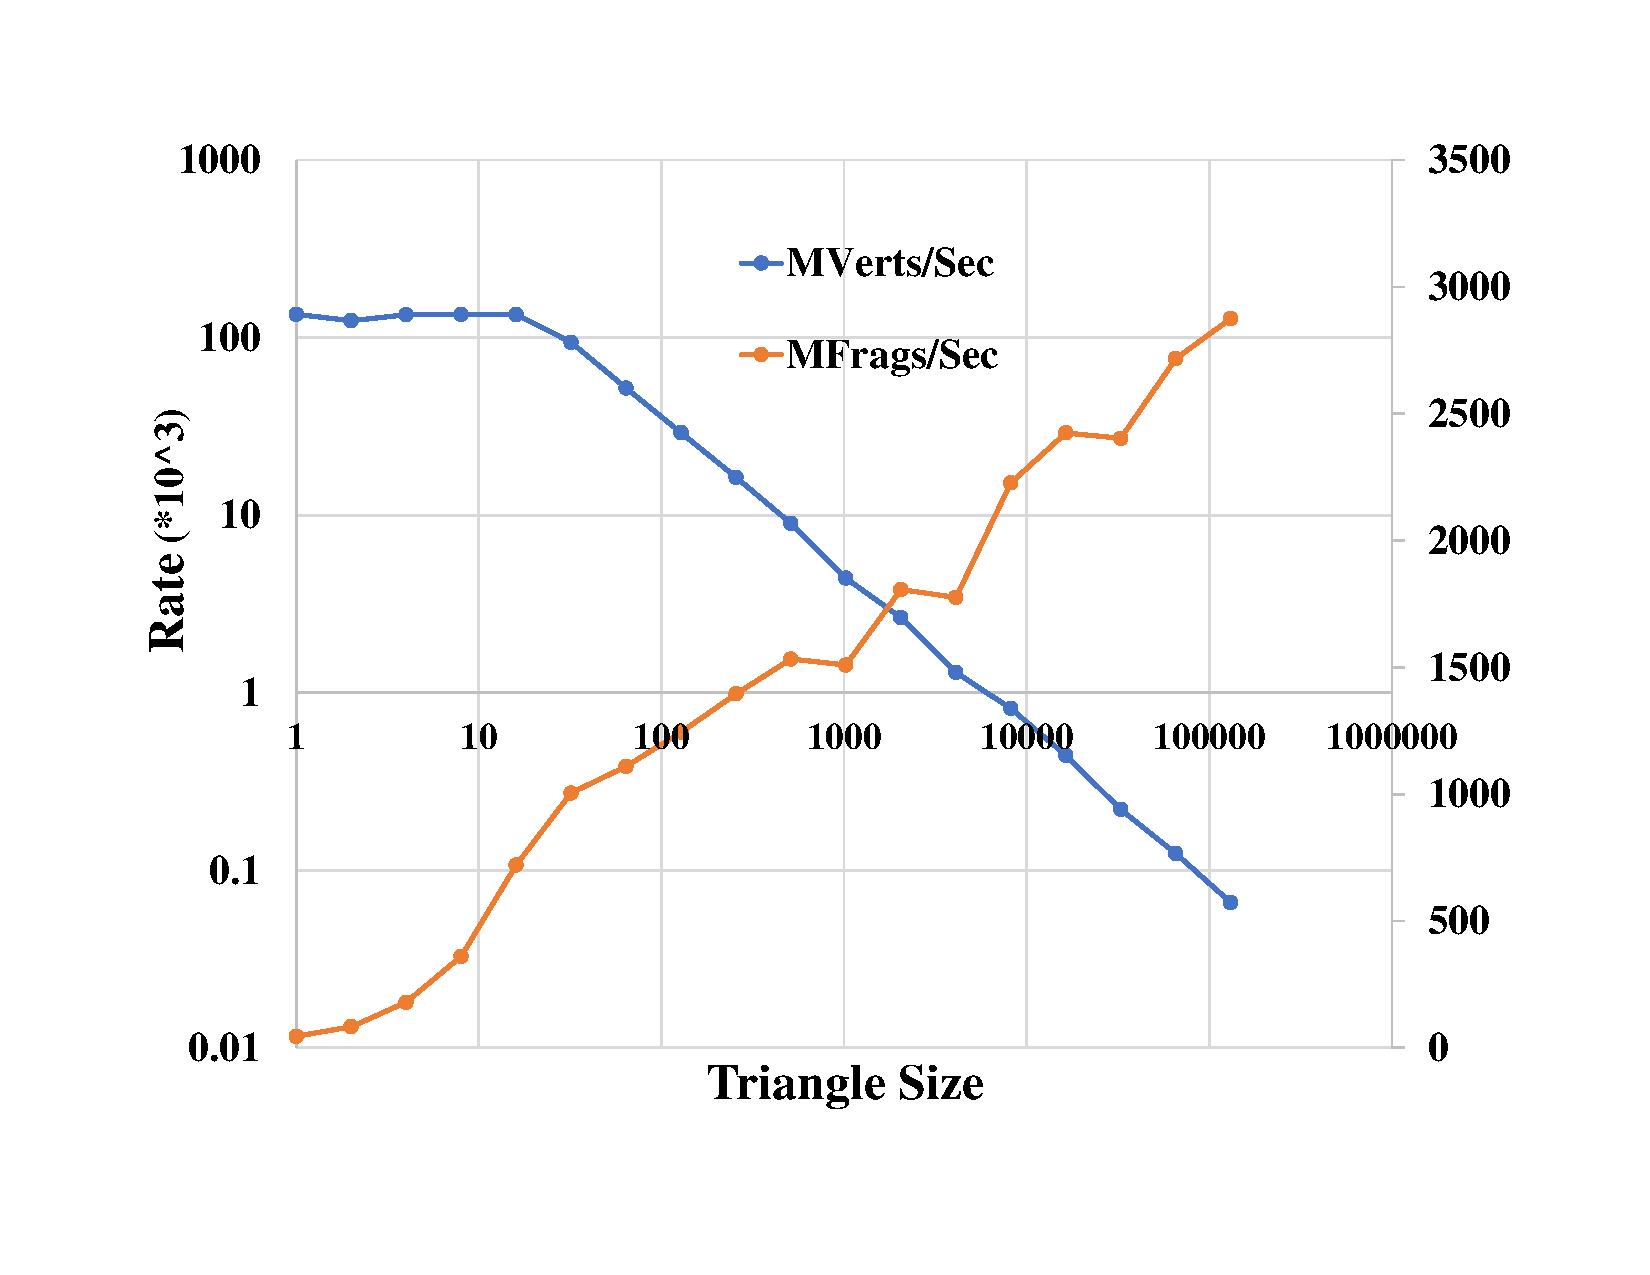
\includegraphics[width=0.49\linewidth]{fig/fill_geo.pdf}}   
 \subfloat[Lit Triangles]
   {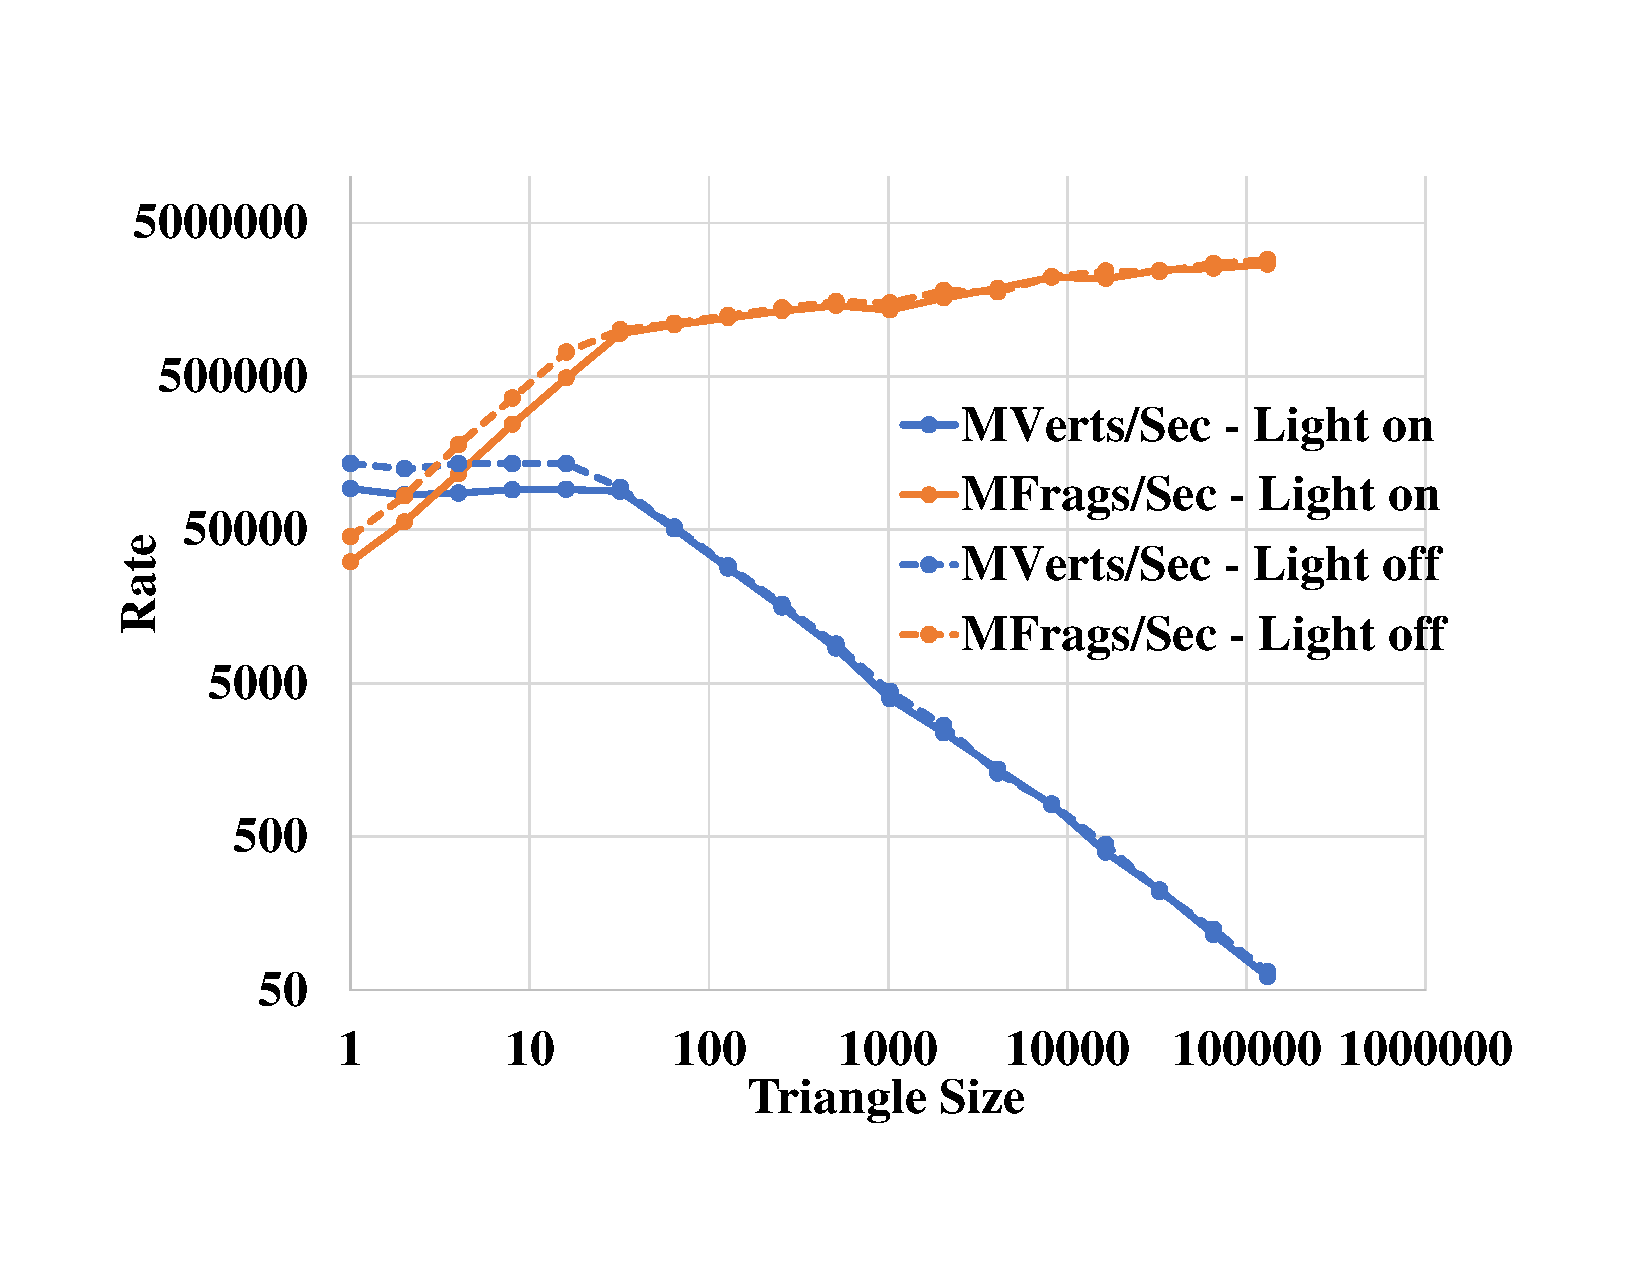
\includegraphics[width=0.49\linewidth]{fig/fill_geo_lit.pdf}}
  \caption{millions of vertices and millions of fragments}
   \label{fig:fill_geo1}
\end{figure} 


\section{Geometry Rate Vs. Fill Rate on Lit Triangles:}
The previous test was done on unlit, untexture triangles which was the default setting. Now we turn on the light on the triangles and do the same test and compare the results with the unlit triangles. The results are shown in Figure \ref{fig:fill_geo1}(b) where the crossover point is almost the same (between triangle size of 2 and 4 pixels). Additionally, we notice that the upper portion of the graph (towards triangle of size greater than 32 pixels) is identical i.e., the dotted and the solid lines overlaps for fill and geometry rates. For the lower part of the graph, it is understood that the geometry will decrease since the lighting is being processed at this stage and thus more work need to done for computing each vertex. This will directly affect the fill rate since less work is sent to the rasterization stage and thus a decline in absolute fill rate. As the triangles get bigger in size, less number of vertices need to be processed in the geometry stage. Thus, even though more work need to be done per vertex, we notice that the unlit triangle rate is almost identical to the lit triangles. Same thing applies for the fill rate; since the geometry stage now is able to send enough work for the rasterization stage, the fill rate is identical for both lit and unlit triangle. 

\begin{figure}[!tbh]
 \centering  
 \subfloat[Textured Triangles]
    {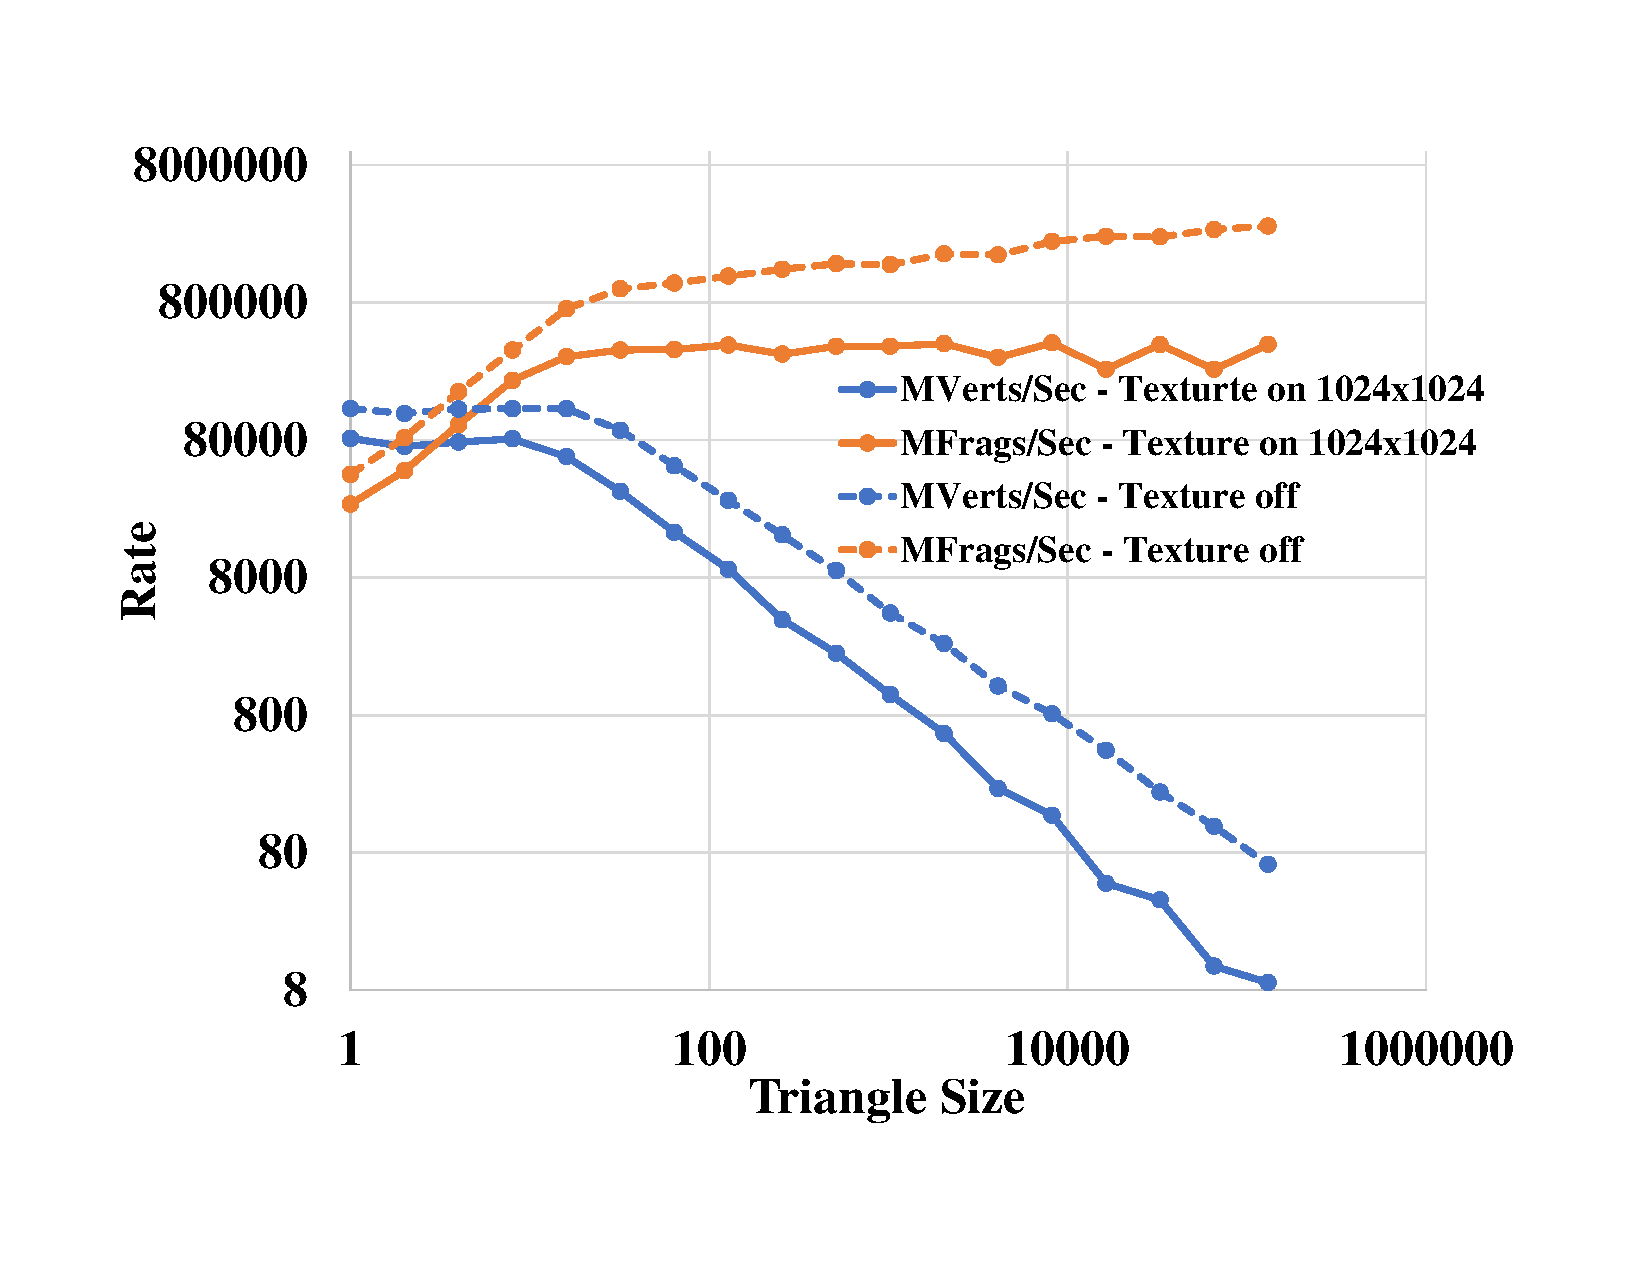
\includegraphics[width=0.49\linewidth]{fig/fill_geo_tx.pdf}}   
 \subfloat[Lit Textured Triangles]
   {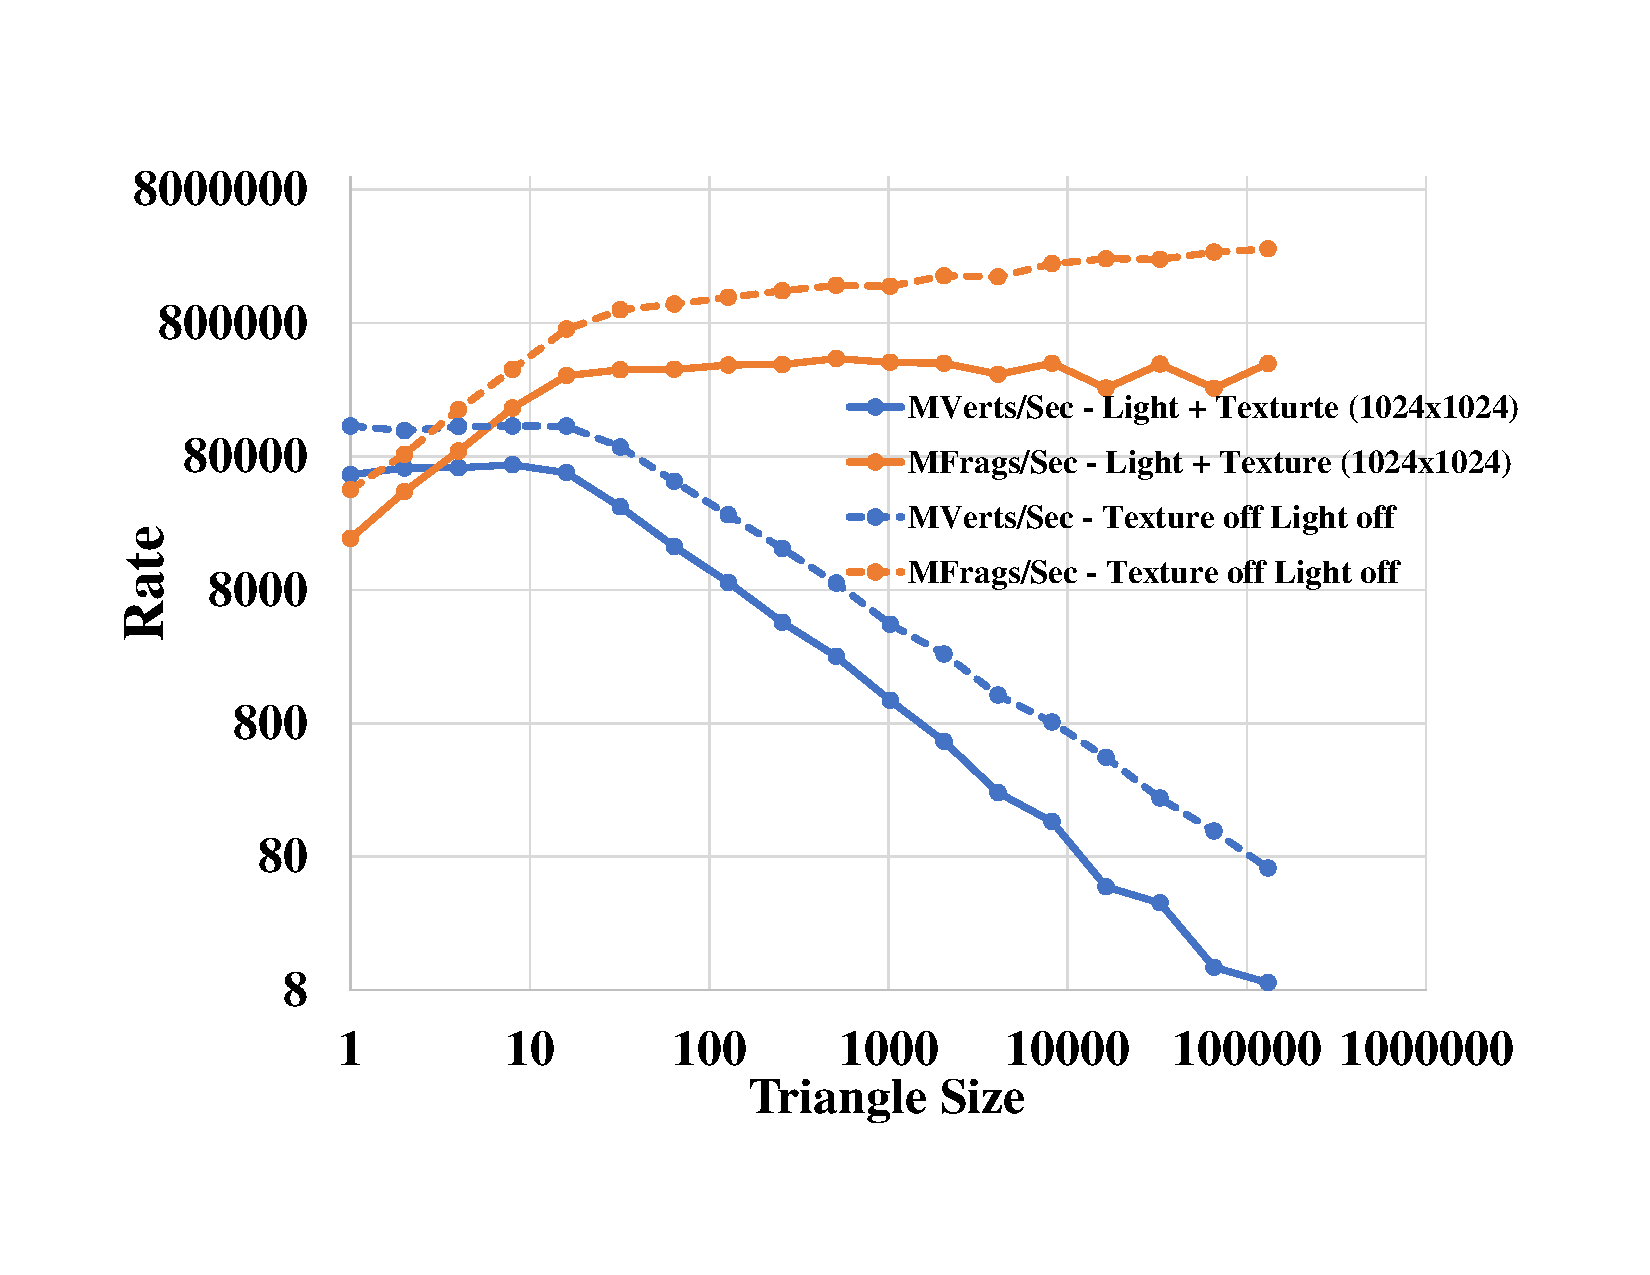
\includegraphics[width=0.49\linewidth]{fig/fill_geo_lit_tx.pdf}}
  \caption{millions of vertices and millions of fragments }
   \label{fig:fill_geo2}
\end{figure} 

\section{Geometry Rate Vs. Fill Rate on Textured Triangles:}



\bibliography{mybib}
\bibliographystyle{plain}

\end{document}
